%%%% fs-run-mapreduce MapReduce transformation on stream

\label {fs-mapreduce}

\begin{figure}[htb]
  \centering
  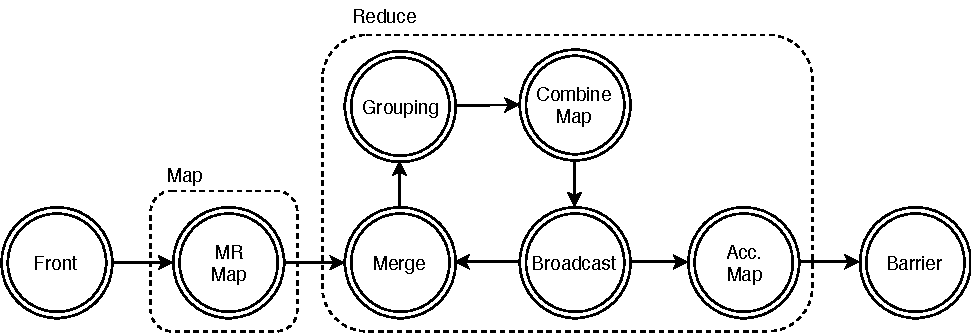
\includegraphics[scale=0.5]{pics/mapreduce}
  \caption{Logical graph for MapReduce transformations}
  \label {mapreduce-graph-figure}
\end{figure}

To show soundness of our model we demonstrate a way to implement MapReduce-like transformation of a stream. Map stage of MapReduce is directly mapped on map operation that extracts a key, but there is a complication with reduce step. Reduce step requires an explicit statate handling. The typical pseudo-code of reduce step is shown on figure 17. It need to store and update current word count.

One possibilitly to implement reduce step in out model is to make business logic state a part of a stream, and work with it as with an ordinary dataitem. Figure~\ref{mapreduce-graph-figure} shows a graph that produces reduced items. Map and reduce parts are highlited with dashed line.

Data items of this stream are: {\it input} items, {\it mapped} items, and {\it reduced} items. Each type of item and the way they were generated are detailed further in this section. However, it is worth to mention that mapped and reduced items have key-value structure of payload. The operations of the stream have the following properties:

\begin{itemize}
\item The first map operation accepts input items and outputs mapped items, according to the business logic. This operation is semantically matched with map step of MapReduce model. Additionally, it should be noted that stream onwards can contain only mapped and reduced items.
\item Merge operation is used for cycle implementation.
\item The window of grouping is set to 2. The hash function is designed to return distinct values for payloads with distinct keys.
\item Filter operation removes tuples with structure \textit{(mapped item; reduced item)}, i.e. tuples, where mapped item was generated before reduced item.
\item The all possible inputs of the second map are the following tuples: \textit{(mapped item), (mapped item; reduced item)}. Any other tuples cannot get in this map because of the filter operation and assumption about the order of items which get in grouping. The first type of input tuples is transformed into reduced item with key inherited from mapped item and some initial value.  The second type is combined into reduce item with the same key. The value of this item is the result of specified reduce function applied to the values of tuple items. Actually, this transformation is equivalent to the reduce step of MapReduce model.
\item Broadcast operation is used to return actual reduced item to grouping and, at the same time, to output it from stream. 
\end{itemize}

According to the provided logical graph, any MapReduce transformation can be implemented using the sequence of map, merge, grouping, filter, and broadcast operations. The key idea is that each reduced item always arrives at grouping right after already combined mapped item and before new one. Hence, each mapped item would be grouped with the actual reduced item. Additionally, when filter accepts tuple {\it (mapped item; reduced item)}, then it means that mapped item was generated before reduced item, and therefore, it had been already combined into the reduced item. The cycle gives ability for new reduced items to get back in grouping operation. Thereby, the stream reacts to each input item by generating new reduced item, which contains the actual value of the reduce step. 

The example of input/output items, which are generated/ transformed by the part of the logical graph, is shown on the figure~\ref {word-count-figure}. This example represents classical MapReduce-based algorithm for word counting. Map step of this algorithm transforms each input word into key-value pair where word is the key, and the value is 1. Reduce step sums all values into the final result for specific key. According to our graph for MapReduce transformations, the item {\it m[dog, 1]} represents mapped item with key "dog" and value 1. The item {\it r[dog, 1]} describes reduced item with key "dog" and value 1. The figure shows how the model reacts on two consequent input items containing word "dog". The meta-information of items is omitted for simplification. More precisely, there are shown 4 stages separated by dotted lines:

\begin{enumerate}
    \item New mapped item with key "dog" arrives at grouping with empty state. Grouping outputs tuple with this single item. Filter accepts the tuple, and Map transforms it to the first reduced item for key "dog" and value 1.
    \item The reduced item arrives at grouping after it went through the cycle. It is grouped in tuple with mapped item that has been already in the state with key "dog". However, filter drops this tuple, because of the order of items.
    \item New mapped item with key "dog" arrives at grouping. It is inserted right after the reduced item in the bucket for key "dog". Grouping outputs tuple containing the reduced item and new mapped item. Filter accepts this tuple, because it has the right order. Map operation combines reduced and mapped items into new reduced items with key "dog" and value 2.
    \item New reduced item arrives at grouping through the cycle, but new generated tuple is not accepted by filter, as well as in the step 2.
\end{enumerate}

\begin{figure}[htb]
  \centering
  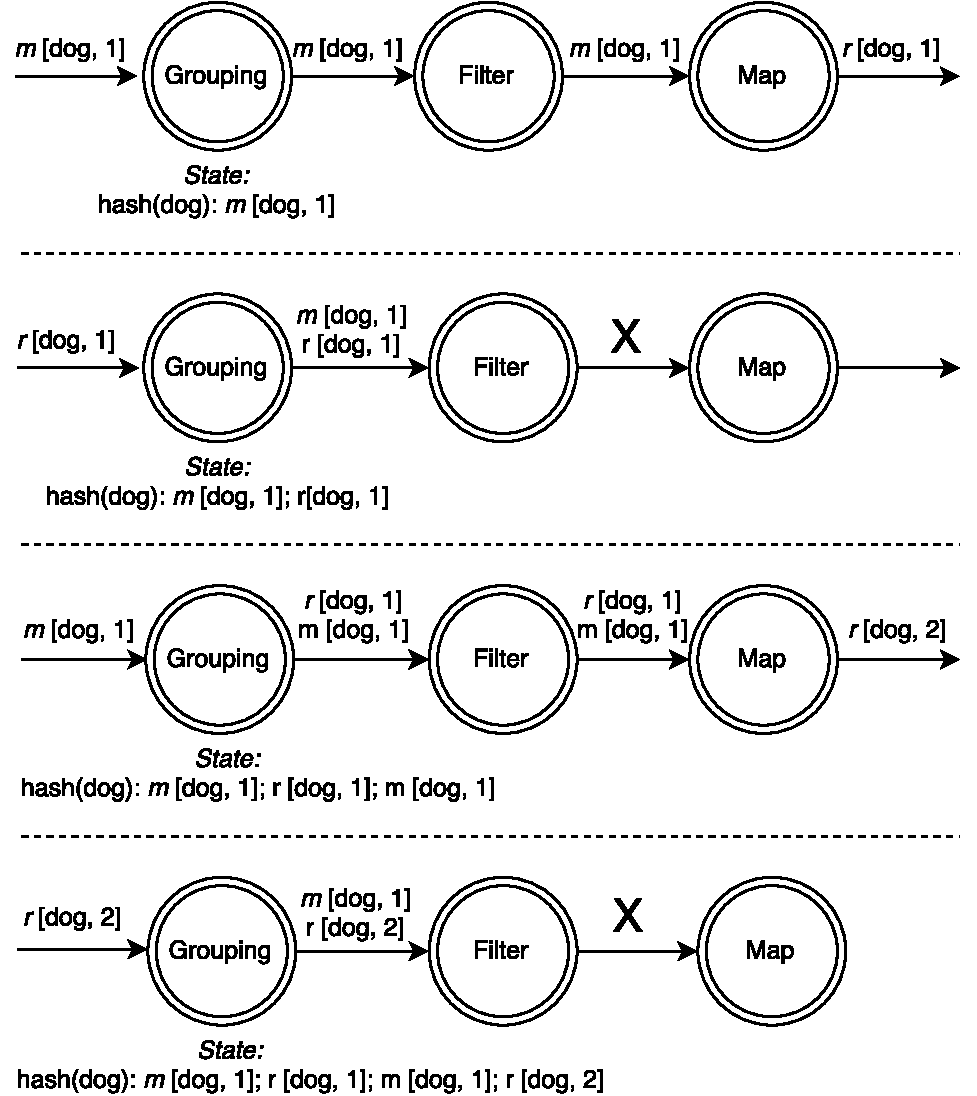
\includegraphics[scale=0.5]{pics/wordcount}
  \caption{Part of the stream evalutaion for word counting}
  \label {word-count-figure}
\end{figure}

